\documentclass[a4paper,12pt]{article}
\usepackage [utf8x]{inputenc}
\usepackage[czech]{babel}
\usepackage{graphicx}
\usepackage{amsmath}
\usepackage{siunitx}
\usepackage{xspace}
\usepackage{url}
\usepackage{indentfirst}
\usepackage[margin=22mm]{geometry}
\usepackage{esvect}
\usepackage{ragged2e}
\usepackage{tikz,pgf}
\usepackage{bm}
\usepackage{perpage}
\usepackage{capt-of}

\graphicspath{
	{img/}
	{plots/}
}

\newcommand{\e}{\text{e}}


\MakeSorted{figure}
\newtoks\jmenopraktika \newtoks\jmeno \newtoks\datum
\newtoks\obor \newtoks\skupina \newtoks\rocnik \newtoks\semestr
\newtoks\cisloulohy \newtoks\jmenoulohy
\newtoks\tlak \newtoks\teplota \newtoks\vlhkost
\jmenopraktika={Paschenův zákon, katodový spád potenciálu v~doutnavém výboji}  % nahradte jmenem vaseho predmetu
\jmeno={Radek Horňák, Lukáš Vrána}            
\datum={15. 3. 2022}        % nahradte datem mereni ulohy                           
\rocnik={2.}                  
\semestr={IV.}                 
\cisloulohy={6}    % cislo ulohy           

\begin{document}
	\begin{center}
		{\Large Přírodovědecká fakulta Masarykovy univerzity} \\
		\bigskip
		{\Large \bfseries PRAKTIKUM Z~FYZIKY PLAZMATU} \\
		\bigskip
		{\Large \the\jmenopraktika}
	\end{center}
	\bigskip
	\noindent
	\setlength{\arrayrulewidth}{1pt}
	\begin{tabular*}{\textwidth}{@{\extracolsep{\fill}} l l}
		\large {\bfseries Zpracovali:}  \the\jmeno  \hspace{20mm} \large  
		{\bfseries Naměřeno:} \the\datum\\[2.5mm]
		\hline
	\end{tabular*}

\section{Teorie}
\subsection{Paschenův zákon}

Z~Townsendovy teorie lavin víme, že působením elektrického pole na zředěný plyn 
dochází k~urychlování přítomných elektronů. Takto urychlené elektrony mohou 
ionizovat neutrální částice a vytvořit takzvanou Townsendovu lavinu. Počet 
elektronů vzniklých v~důsledku Townsendovy laviny závisí exponenciálně na dráze 
$d$  

\begin{equation}
	n = n_0\,\e^{\alpha d}
	\label{1}
\end{equation}
kde $n_0$ je počet elektronů v~počátečním bodě $d = 0$ a $\alpha$ je první 
Townsendův nebo také ionizační koeficient. Elektrické pole můžeme 
charakterizovat napětím $U$ přiloženým mezi dvě rovinné elektrody, dráha $d$ je 
vzdálenost mezi elektrodami. Elektronovou lavinu doprovází vznik iontů, jejichž 
počet lze vyjádřit jako

\begin{equation}
	 n_\text{i} = n_0\,(\e^{\alpha d}-1)
	\label{2}
\end{equation}

Ionty jsou polem urychlovány ke katodě, dopadají na ni a vyvolávají sekundární 
emisi elektronů. Tu popisuje Townsendův třetí koeficient neboli koeficient 
sekundární emise $\gamma$. Konkrétně udává průměrný počet elektronů emitovaných 
jedním iontem při jeho dopadu na katodu. Pomocí $\gamma$ lze vyjádřit podmínku 
zapálení výboje jako

\begin{equation}
	\gamma\,(\e^{\alpha d } - 1) = 1
	\label{3}
\end{equation} 
tedy že v~lavině musí být jedním primárním elektronem vytvořeno tolik iontů, 
které dopadem na katodu způsobí emisi jednoho nového elektronu. Ionizační 
koeficient $\alpha$ závisí na intenzitě elektrického pole 

\begin{equation}
	\frac{\alpha}{p} = A\,\e^{-\frac{Bp}{E}} 
	\label{4}
\end{equation}
kde $A = 1/\lambda_1$ a $B = U/\lambda_1$ jsou konstanty závislé na druhu 
plynu, $\lambda_1$ je střední volná dráha elektronů při jednotkovém tlaku. Dále 
lze (\ref{4}) přepsat jako

\begin{equation}
	\frac{\alpha}{p} = A\,\e^{-\frac{Bpd}{U}} 
	\label{5}
\end{equation}
Logaritmováním a úpravou (\ref{5}) získáme

\begin{equation}
	U~= \frac{B\,pd}{\ln A~- \ln \frac{\alpha}{d}}
	\label{6}
\end{equation}
Zápalné napětí výboje $U_\text{z}$ získáme dosazením $d\alpha$ z~(\ref{6}) do 
podmínky zápálení výboje (\ref{3}). Logaritmováním a dalšími úpravami 
dojdeme k~tvaru

\begin{equation}
	A\,pd\,\e^{-\frac{Bpd}{U_\text{z}}} = \ln \left(\frac{1}{\gamma} + 1\right)
	\label{7}
\end{equation}
Pro daný plyn a materiál katody položme pravou stranu

\begin{equation}
	\ln \left(\frac{1}{\gamma} + 1\right) = C
	\label{8}
\end{equation}
Úpravami dostáváme

\begin{equation}
	U_\text{z} = \frac{B\,pd}{C' + \ln(pd)}
	\label{9}
\end{equation}
kde $C' = \ln C - \ln A$. Závislost $U_\text{z} = f (pd)$ se nazývá Paschenův 
zákon. 
Má charakteristický tvar, včetně minima nazývaného Stoletovův bod.


\subsection{Doutnavý výboj}
Doutnavý výboj je druh výboje, jehož typický vzhled můžeme vidět na schématu na 
obr.~\ref{glowdischarge}. V~rozmezí tlaku 10$^1$-10$^2$\,\si{\pascal} v~něm 
můžeme 
pozorovat střídající se temné nebo svítící oblasti. Elektron pohybující se ve 
výboji od katody k~anodě získá dostatečnou energii k~excitaci neutrálů až 
v~oblasti katodové vrstvy, ta je tedy první svítící oblastí. Následuje temný 
katodový prostor. Zde mají elektrony energii vyšší, a nedochází tak často k 
excitaci a vzniku fotonů. Na konci temného katodového prostoru mají elektrony 
dostatečnou energii k ionizaci plynu. Nové elektrony s malou energií, které 
vznikly ionizací, vytvoří další svítivou oblast, kterou nazýváme záporné 
světlo. Energie elektronů dále klesá a následuje Faradayův temný prostor. Na 
jeho konci vzrůstá intenzita elektrického pole, energie elektronů opět roste a 
jsou schopné excitačních svítivých srážek, viz kladný sloupec. Jak se blížíme 
k~anodě, na konci kladného sloupce vzniká anodový spád potenciálu v~důsledku 
prostorového náboje, elektrony vystupují z~kladného sloupce s~malou rychlostí. 
Jakmile překonají anodový temný prostor, mají opět dostatek energie na excitaci 
i ionizaci neutrálů, a tak u~anody pozorujeme anodové světlo.

\begin{figure}[h]
	\centering
	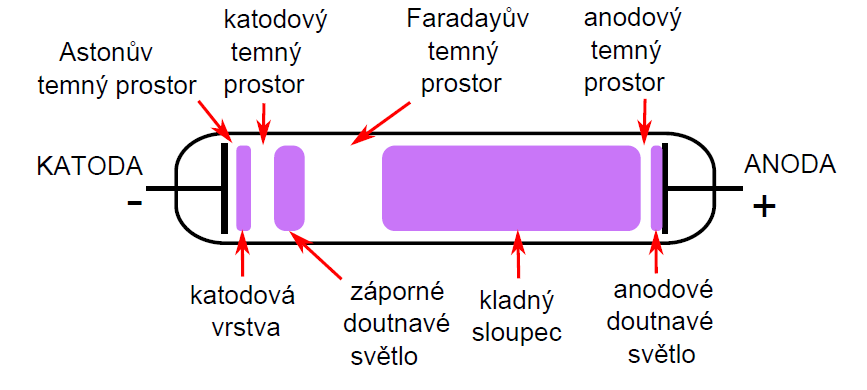
\includegraphics[width=130mm]{glowdischarge.png}
	\caption{Schéma doutnavého výboje.}
	\label{glowdischarge}
\end{figure}

Výboj můžeme charakterizovat voltampérovou (VA) charakteristikou. Ta pro 
samostatný výboj je vidět na obr. \ref{VA}. Za změnu proudu při konstantním 
napětí u~bodu B je zodpovědný prostorový náboj, kvůli němuž dojde ke změně 
původního elektrického pole. To nové může podporovat ionizaci ve výboji, což 
způsobí další růst proudu, přičemž napětí na elektrodách může klesat, a vznikne 
tak část charakteristiky mezi body B a C. Specifická oblast charakteristiky je 
mezi body C a D, zvyšování proudu zde nelze vysvětlit nárůstem driftové 
rychlosti nabitých částic. Musí se zde měnit celkový počet částic 
procházejících průřezem výbojky. Celkový počet částic $N$ lze napsat jako

\begin{equation}
	N = \int n \text{d}S
	\label{10}
\end{equation}
kde $n$ je koncentrace nabitých částic ve výboji a $S$ je plocha, kterou zabírá 
záporné světlo na katodě. V~katodové oblasti normálního doutnavého výboje 
vzrůstá $N$ v~důsledku růstu $S$, v~kladném sloupci však vzrůstá koncentrace 
$n$. Napětí ve výbojce se skládá z~napětí v~katodové oblasti a ze spádu napětí 
na kladném sloupci, který se s~rostoucím proudem zvyšuje. Pokud vzroste proud 
tak, že celá katoda je pokryta záporným světlem, přechází doutnavý výboj do 
takzvaného anomálního stavu. Napětí v~katodové oblasti roste rychleji než 
napětí v~kladném sloupci klesá, výsledkem je oblast charakteristiky od bodu D 
k~E. Oblast E-F odpovídá přechodu na obloukový výboj.

\subsection{Katodový spád potenciálu v~doutnavém výboji}
Katodový spád potenciálu $U_\text{k}$ je označení pro napětí mezi ostrou 
hranicí záporného světla a katodou. Je funkcí materiálu elektrod a plynu ve 
výbojce. Stanovení katodového spádu potenciálu lze provést metodou ztíženého 
výboje. 
Tato metoda spočívá v~udržování konstantního výbojového proudu, přičemž se mění 
vzdálenost elektrod a na ní závislé napětí. Zmenšováním vzdálenosti elektrod se 
zmenšuje kladný sloupec a následně Faradayův temný prostor. Dalším 
zmen\-šo\-vá\-ním vzdálenosti elektrod začne napětí nutné na 
udržení výboje prudce růst, protože elektronové laviny nemají k~dispozici 
potřebnou dráhu pro dostatečnou ionizaci.

\begin{figure}[h]
	\centering
	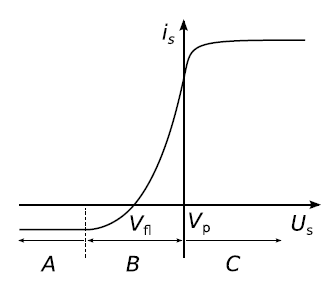
\includegraphics[width=130mm]{VA.png}
	\caption{Voltampérová charakteristika samostatného výboje.}
	\label{VA}
\end{figure}




\section{Měření a výsledky}
\subsection{Paschenův zákon}
Pro měření použijeme výbojku s~pohyblivými elektrodami, viz schéma na 
obr.~\ref{schema1}. Tlak měříme Piraniho 
manometrem, zápalné napětí určujeme voltmetrem s~vysokým vstupním odporem. Plyn 
ve výbojce je vzduch, kalibrační faktor k~Piraniho manometru je tedy 1. První 
měření provedeme s~konstantním tlakem $p = 100\,\si{\pascal}$, přičemž budeme 
měnit vzdálenost elektrod od 4\,\si{\milli\meter} do 50\,\si{\milli\meter}. Na 
výbojce zvyšujeme napětí a odečítáme hodnotu napětí v~okamžiku zapálení výboje. 
Mezi každým měřením vyčkáváme alespoň jednu minutu na rekombinaci náboje ve 
výbojce. Výsledný graf závislosti $U_\text{z} = f(pd)$ je na 
obr.~\ref{tlakfixed}. 
Body jsou proloženy funkcí podle rovnice~(\ref{9}) a získané hodnoty $B$ 
a $C'$ jsou v~tabulce~\ref{tab1}. Výsledky měření se od ideální závislosti 
popsané 
rovnicí~(\ref{9}) odchylují. Tato ochylka může být způsobena jak 
nepřesností odečítání zápalného napětí, tak nedostatečnou rekombinací nábojů 
mezi jednotlivými měřeními. 
%440,68\pm94,46
Druhá série měření je za konstantní vzdálenosti elektrod $d = 
20\,\si{\milli\meter}$, 
měníme tlak od 25\,\si{\pascal} do 300\,\si{\pascal}. Opět zapisujeme hodnotu 
napětí v~okamžiku zapálení výboje. Graf závislosti $U_\text{z} = f(pd)$ je na 
obr.~\ref{dfixed}. Body jsou proloženy funkcí podle rovnice~(\ref{9}), získané 
konstanty 
$B$ a $C'$ jsou uvedeny v~tabulce~\ref{tab1}. Toto měření se oproti 
předchozímu více 
blíží ideální závislosti popsané rovnicí~(\ref{9}), z~grafu vidíme až na malou 
odchylku typickou závislost napětí na součinu tlaku a vzdálenosti elektrod.
Z minim fitovaných křivek je v~tabulce~\ref{tab1} také uvedeno zápalné napětí 
$U_\text{z,min}$ a 
součin tlaku a vzdálenosti $pd_{\text{min}}$. Tyto hodnoty 
lze srovnat s~tabulkovými hodnotami \cite{wiki}, které se uvádí pro vzduch: 
$U_\text{z,min} = 327$\,V a $pd_{\text{min}} = 0,75$\,Pa$\cdot$m.
%286,26\pm27,22
% UZ ZJISTIT A OKOMENTOVAT, Z MINIMA FCE NEBO MĚŘENÍ?

%\begin{center}
%	\begin{table}[h]
%		\centering
%		\caption{Hodnoty konstant $B$ a $C'$}
%		\label{tab1}
%		\begin{tabular}{|c|c|c|c|} \hline
%			\multicolumn{2}{|c|}{Měření s~konstantním tlakem} 
%			& \multicolumn{2}{c|}{Měření s~konstantní vzdáleností elektrod}  \\ 
%\hline
%			$B$ [\si{\meter\squared\per\coulomb}] & $C'$ 
%			& $B$ [\si{\meter\squared\per\coulomb}] & $C'$ \\ \hline
%			310 $\pm$ 30 & 1,05 $\pm$ 0,02 &  290 $\pm$ 30  
%			& 0,79 $\pm$ 0,01 \\ \hline
%			$U_\text{z}$\,[V] & $pd$\,[Pa$\cdot$m] & $U_\text{z}$\,[V] & 
%$pd$\,[Pa$\cdot$m]
%			\\ \hline
%			$291,6$ & 0,95 & 351,4 & 1,23 \\ \hline
%
%		\end{tabular}
%	\end{table}
%\end{center}

\begin{figure}[h!]
	\centering
	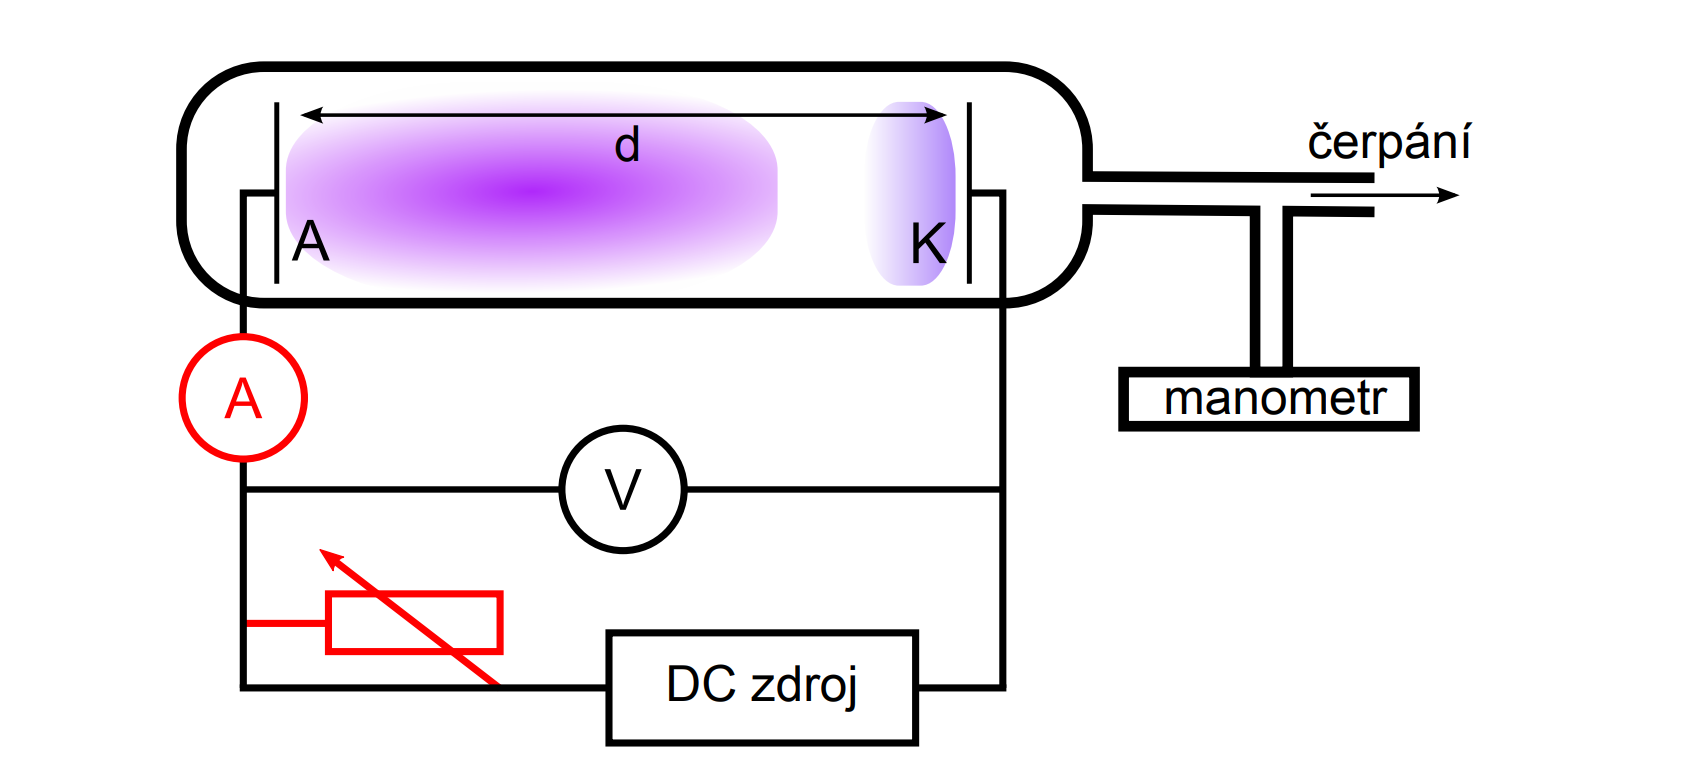
\includegraphics[width=145mm]{schema1.png}
	\caption{Schéma zapojení pro měření Paschenovy křivky. Červeně zvýrazněné 
		prvky jsou zapojeny v části praktika pro měření voltamperové 
		charakteristiky.}
	\label{schema1}
\end{figure}

\begin{center}
\begin{table}[h]
	\centering
	\caption{Hodnoty konstant $B$, $C'$, zápalného napětí $U_\text{z,min}$ a 
	minima 
	součinu $pd_{\text{min}}$}
	\label{tab1}
	\begin{tabular}{|r|c|c|c|c|}
		\hline
		\multicolumn{1}{|l|}{}                                                  
		           	&$B$\,[\si{\volt\per\pascal\per\meter}] & $C'$  & 
		           	$U_\text{z,min}$\,[V]    & 
		           	$pd_{\text{min}}$\,[Pa$\cdot$m]   \\ \hline
		\begin{tabular}[c]{@{}r@{}}Měření s konstantním\\  
		tlakem\end{tabular}               & 310 $\pm$ 30 & 1,05 $\pm$ 0,02 & 
		291,6 & 0,95 
		\\ \hline
		\begin{tabular}[c]{@{}r@{}}Měření s konstantní \\ vzdáleností 
		elektrod\end{tabular} & 290 $\pm$ 30 & 0,79 $\pm$ 0,01 & 351,4 & 1,23 
		\\ \hline
	\end{tabular}
\end{table}
\end{center}

\begin{figure}[h!]
	\centering
	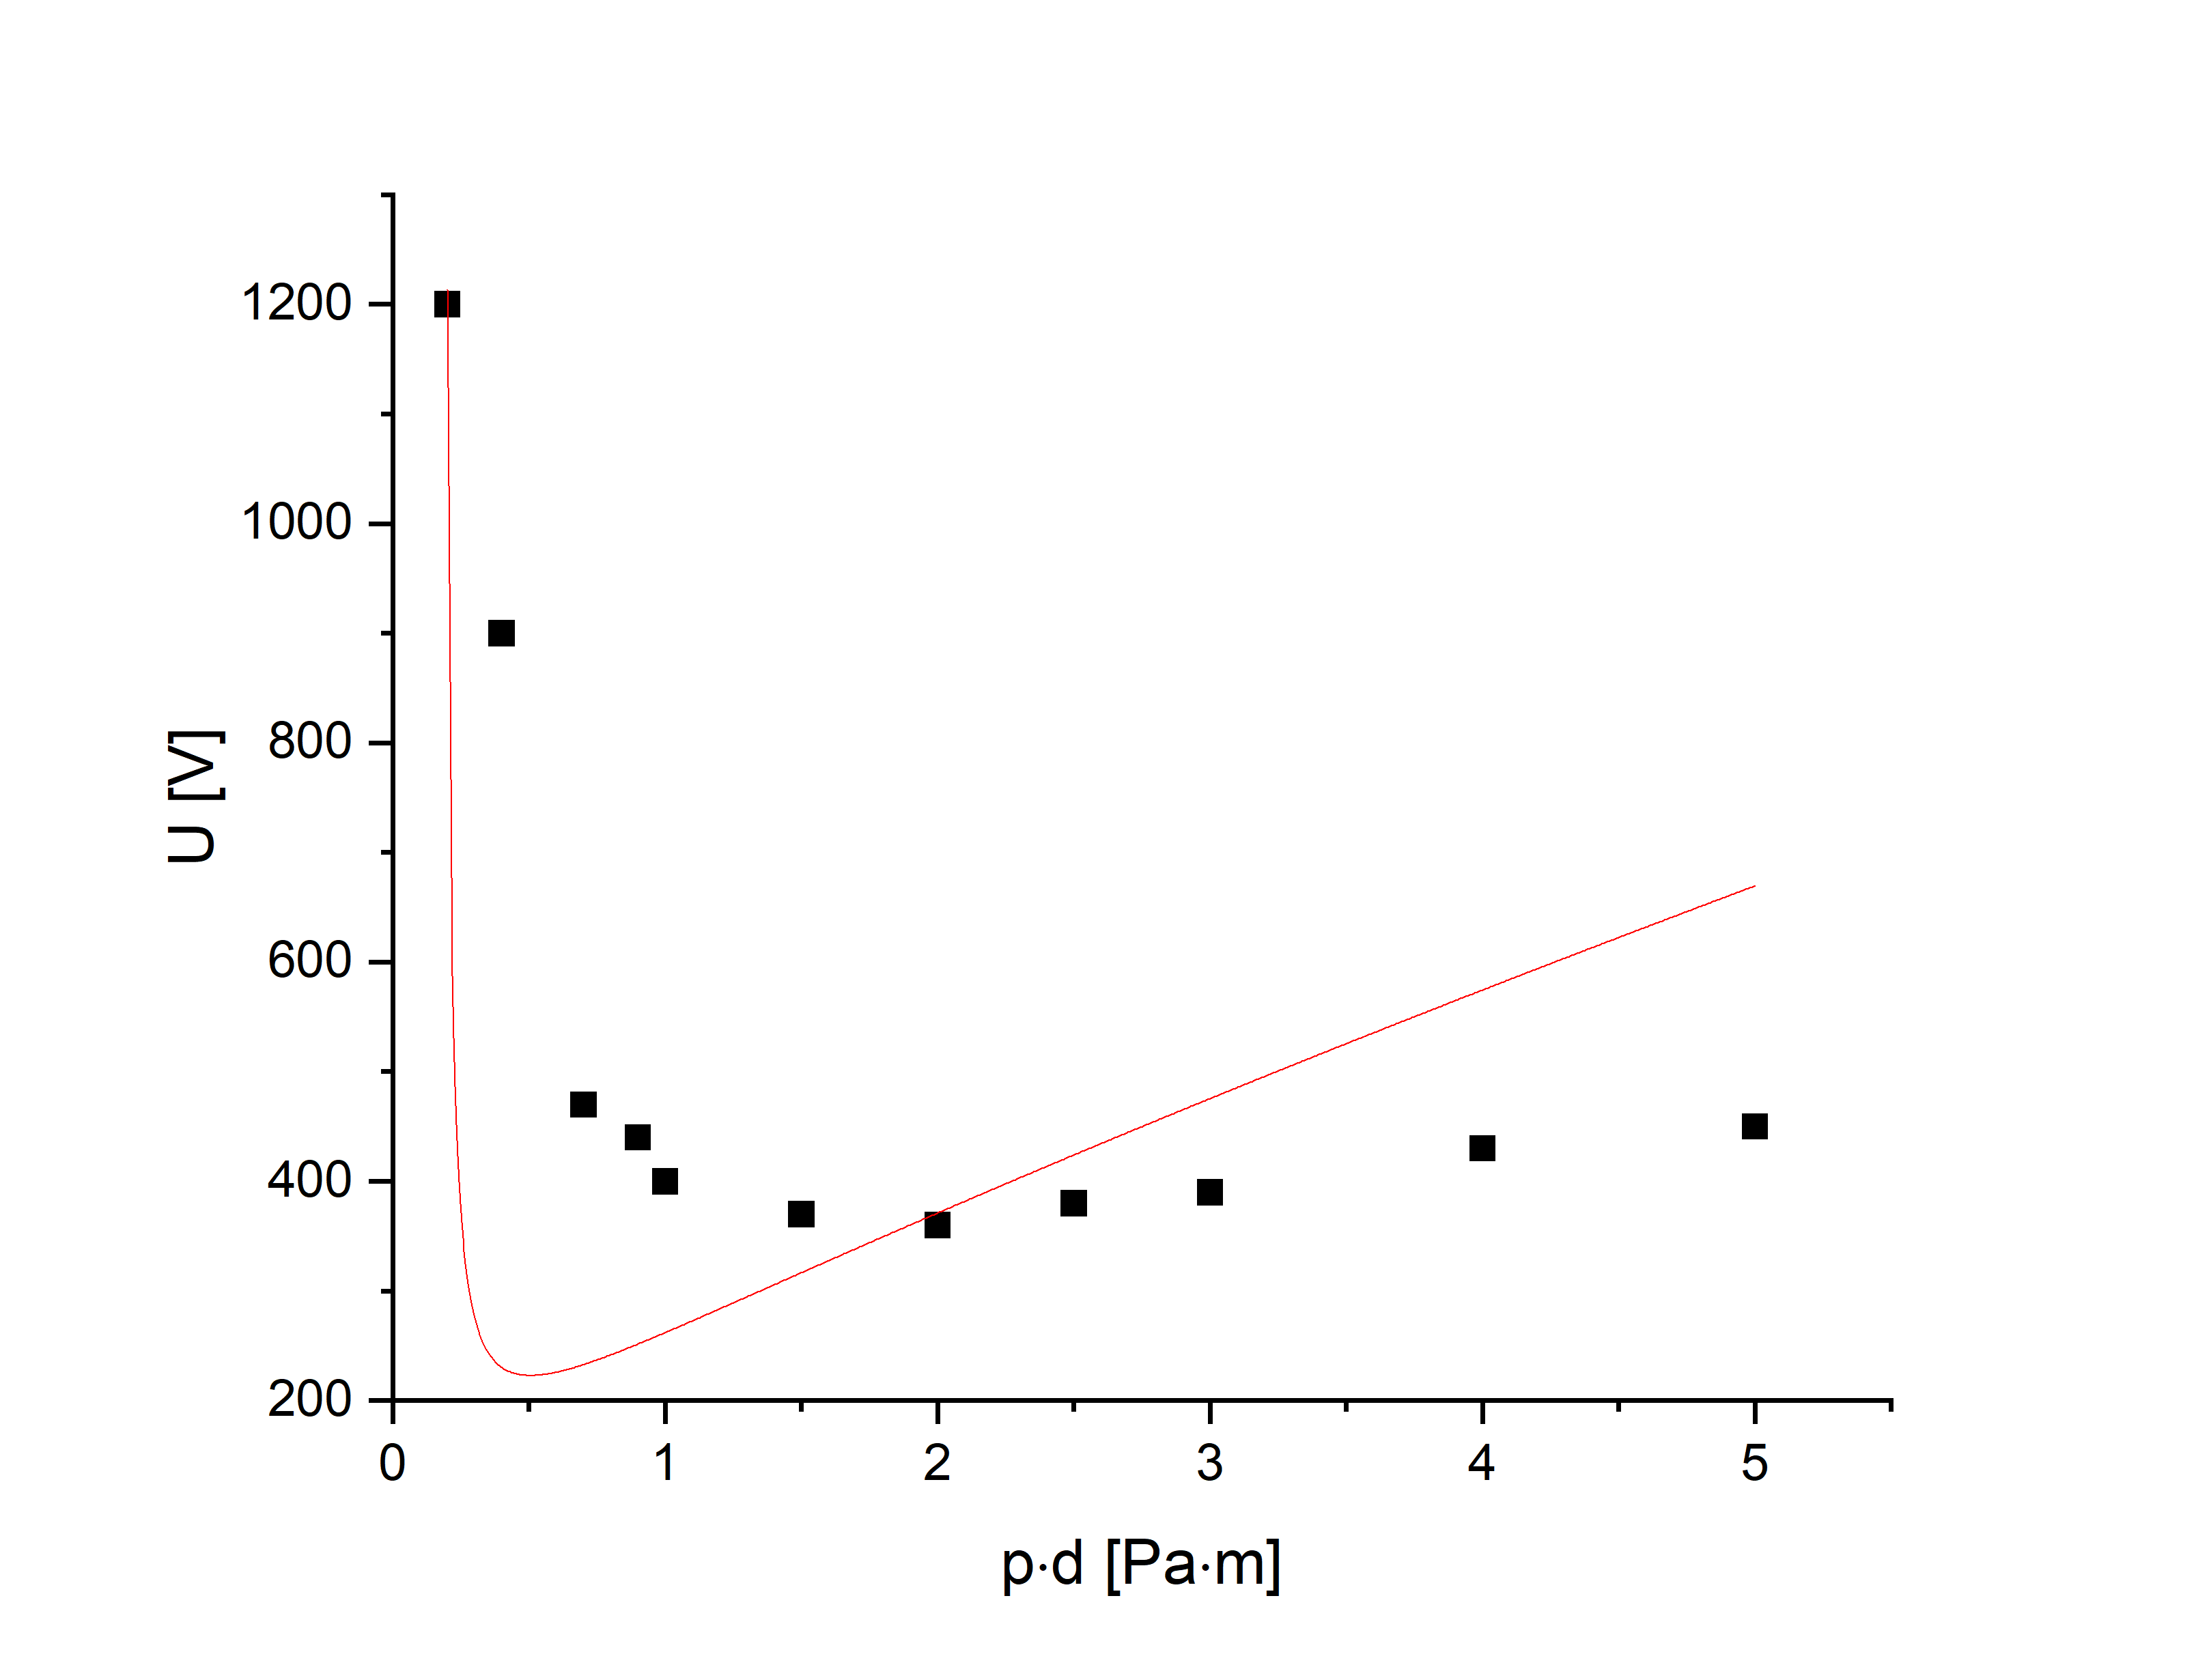
\includegraphics[width=150mm]{tlakfixed.png}
	\caption{Naměřená Paschenova křivka při konstantním tlaku.}
	\label{tlakfixed}
\end{figure}


\begin{figure}[h!]
	\centering
	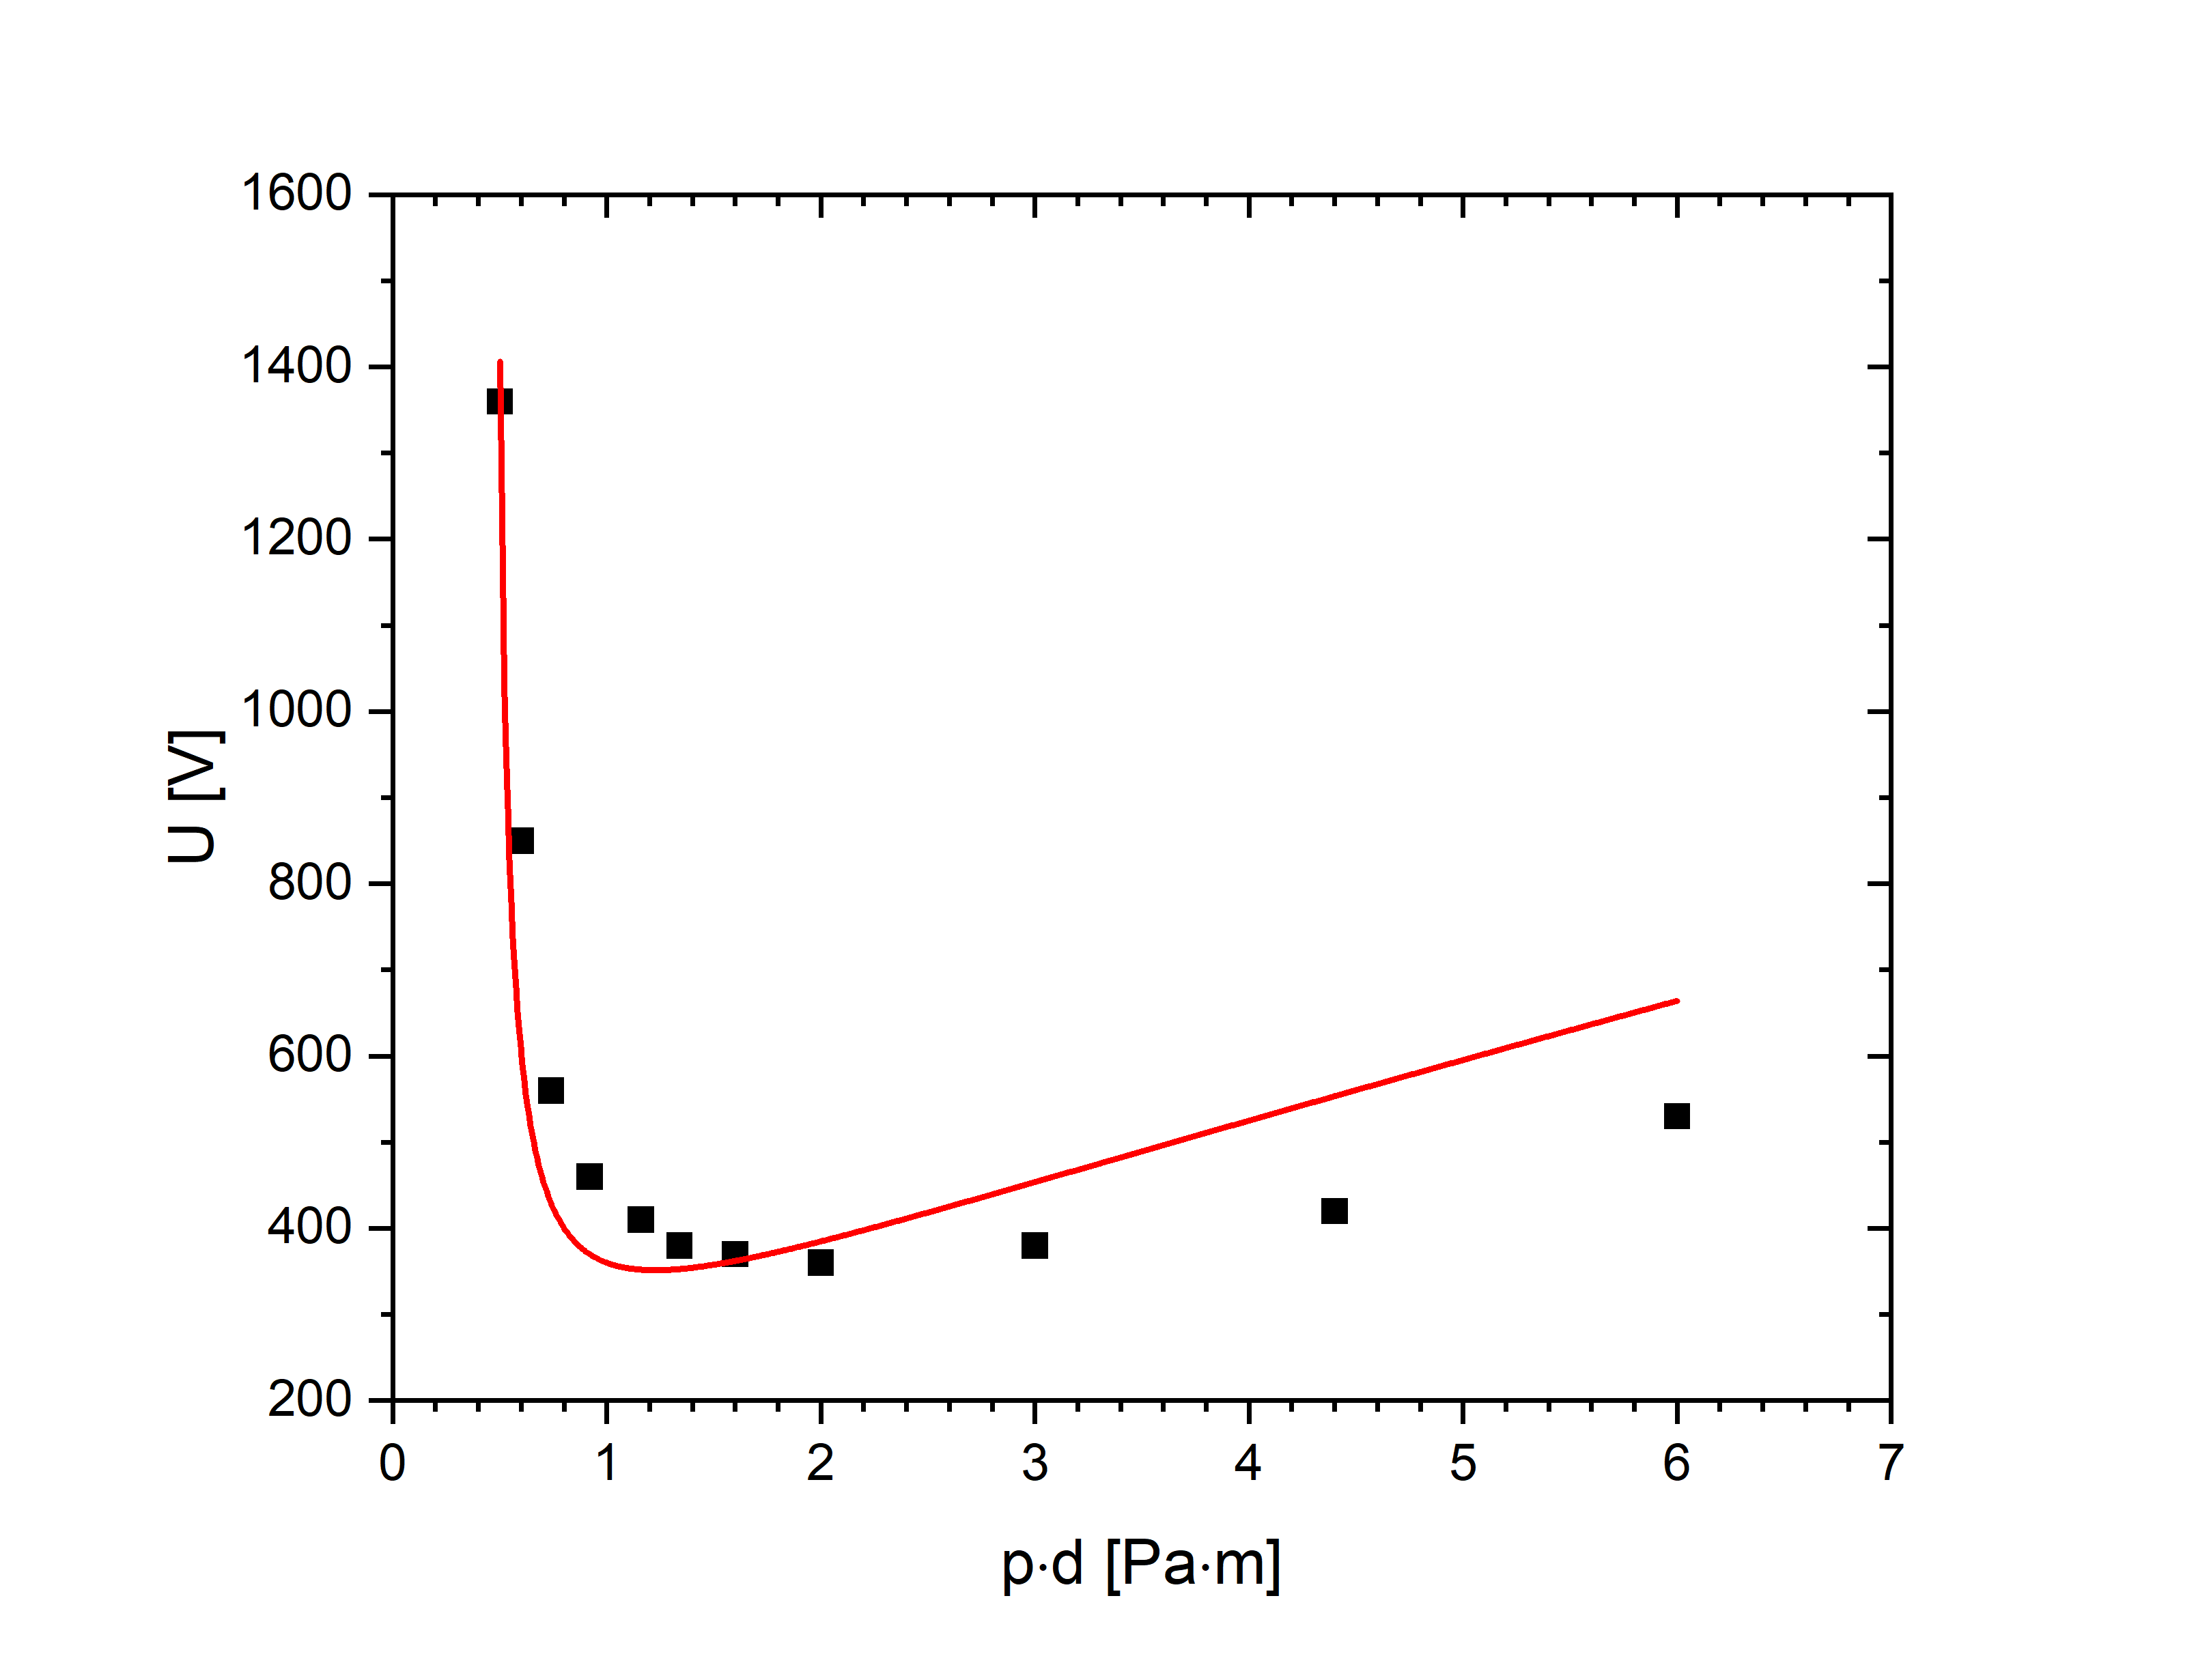
\includegraphics[width=150mm]{dfixed.png}
	\caption{Naměřená Paschenova křivka při konstantní vzdálenosti elektrod.}
	\label{dfixed}
\end{figure}

\clearpage
\subsection{Katodový spád potenciálu v~doutnavém výboji}
Měření katodového spádu potenciálu metodou ztíženého výboje provedeme pro dvě konstantní hodnoty tlaku a proudu, 
zaznamenáváme změnu napětí se změnou vzdálenosti elektrod při konstantním 
proudu, viz schéma na obr.~\ref{schema2v2}. V~grafu na 
obr.~\ref{KatodovySpad} jsou vidět naměřené závislosti. Výsledné hodnoty 
katodového spádu jsou uvedeny v~tabulce~\ref{tab2}. S~vyšším proudem i tlakem
jsme naměřili nižší katodový spád. Při měření jsme vypozorovali, 
že katodová vrstva se s~rostoucím tlakem vizuálně ztenšuje. Dle literatury je 
katodový spád nejvyšší pro největší průřez katodové vrstvy, tedy v~případě, 
když je 
celý povrch katody pokrytý výbojem. To je v~souladu s~našimi pozorováními. 
Při změně tlaku pozorujeme v grafu také posun minima, který odpovídá Paschenovu 
zákonu, 
tedy při vyšším tlaku se minimum posunulo k menší vzdálenosti elektrod.  

%komentář proč se katodový spád liší
%komentář vizuál výboje
	  

%co ty tři body vlevo 

\begin{figure}[h!]
	\centering
	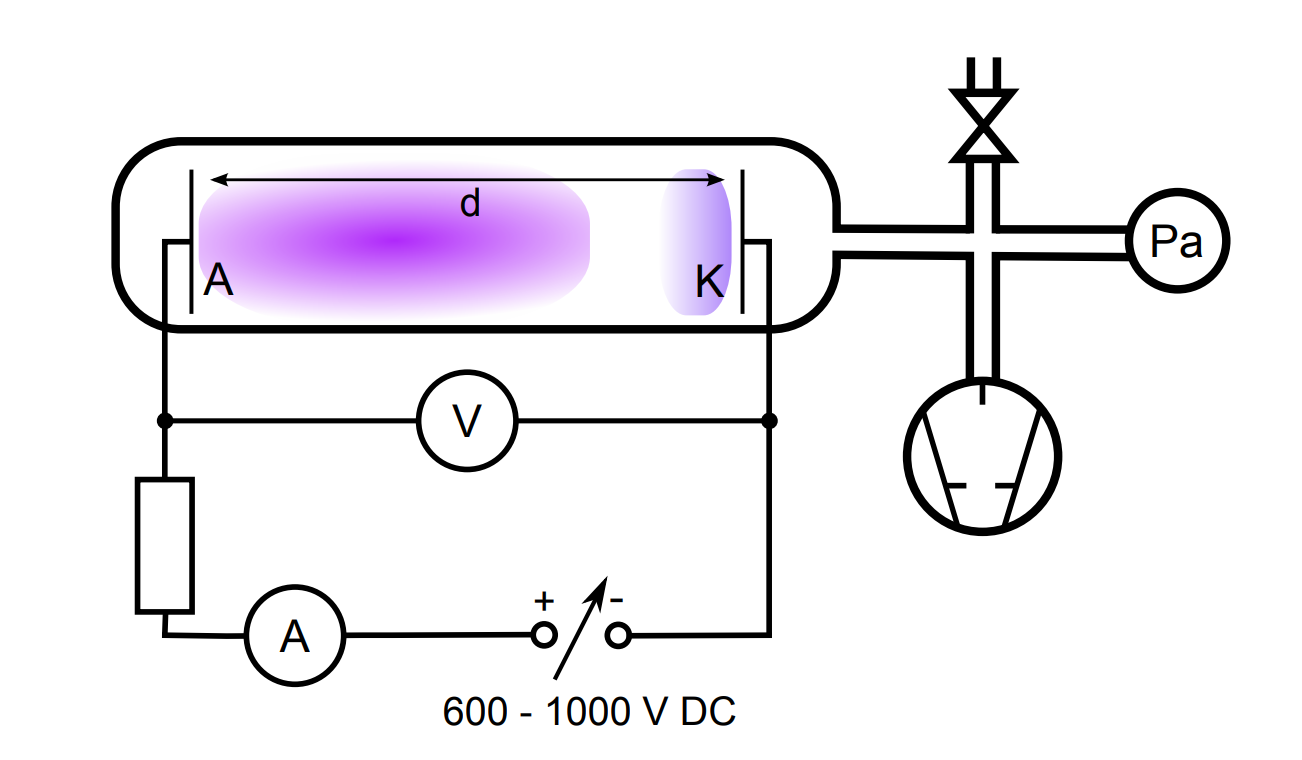
\includegraphics[width=145mm]{schema2v2.png}
	\caption{Schéma zapojení pro měření katodového spádu potenciálu.}
	\label{schema2v2}
\end{figure}

\begin{center}
	\begin{table}[h!]
		\centering
		\caption{Naměřené hodnoty katodového spádu}
		\label{tab2}
		\begin{tabular}{|c|c|} \hline
			$I = 1\,\si{\milli\ampere}$, $p = 33\,\si{\pascal}$ 
			& $I = 1,8\,\si{\milli\ampere}$, $p = 100\,\si{\pascal}$\\ \hline
			$U_\text{k}$ [V] & $U_\text{k}$ [V]\\ \hline
			701 & 514 \\ \hline
			
		\end{tabular}
	\end{table}
\end{center}

\begin{figure}[h!]
	\centering
	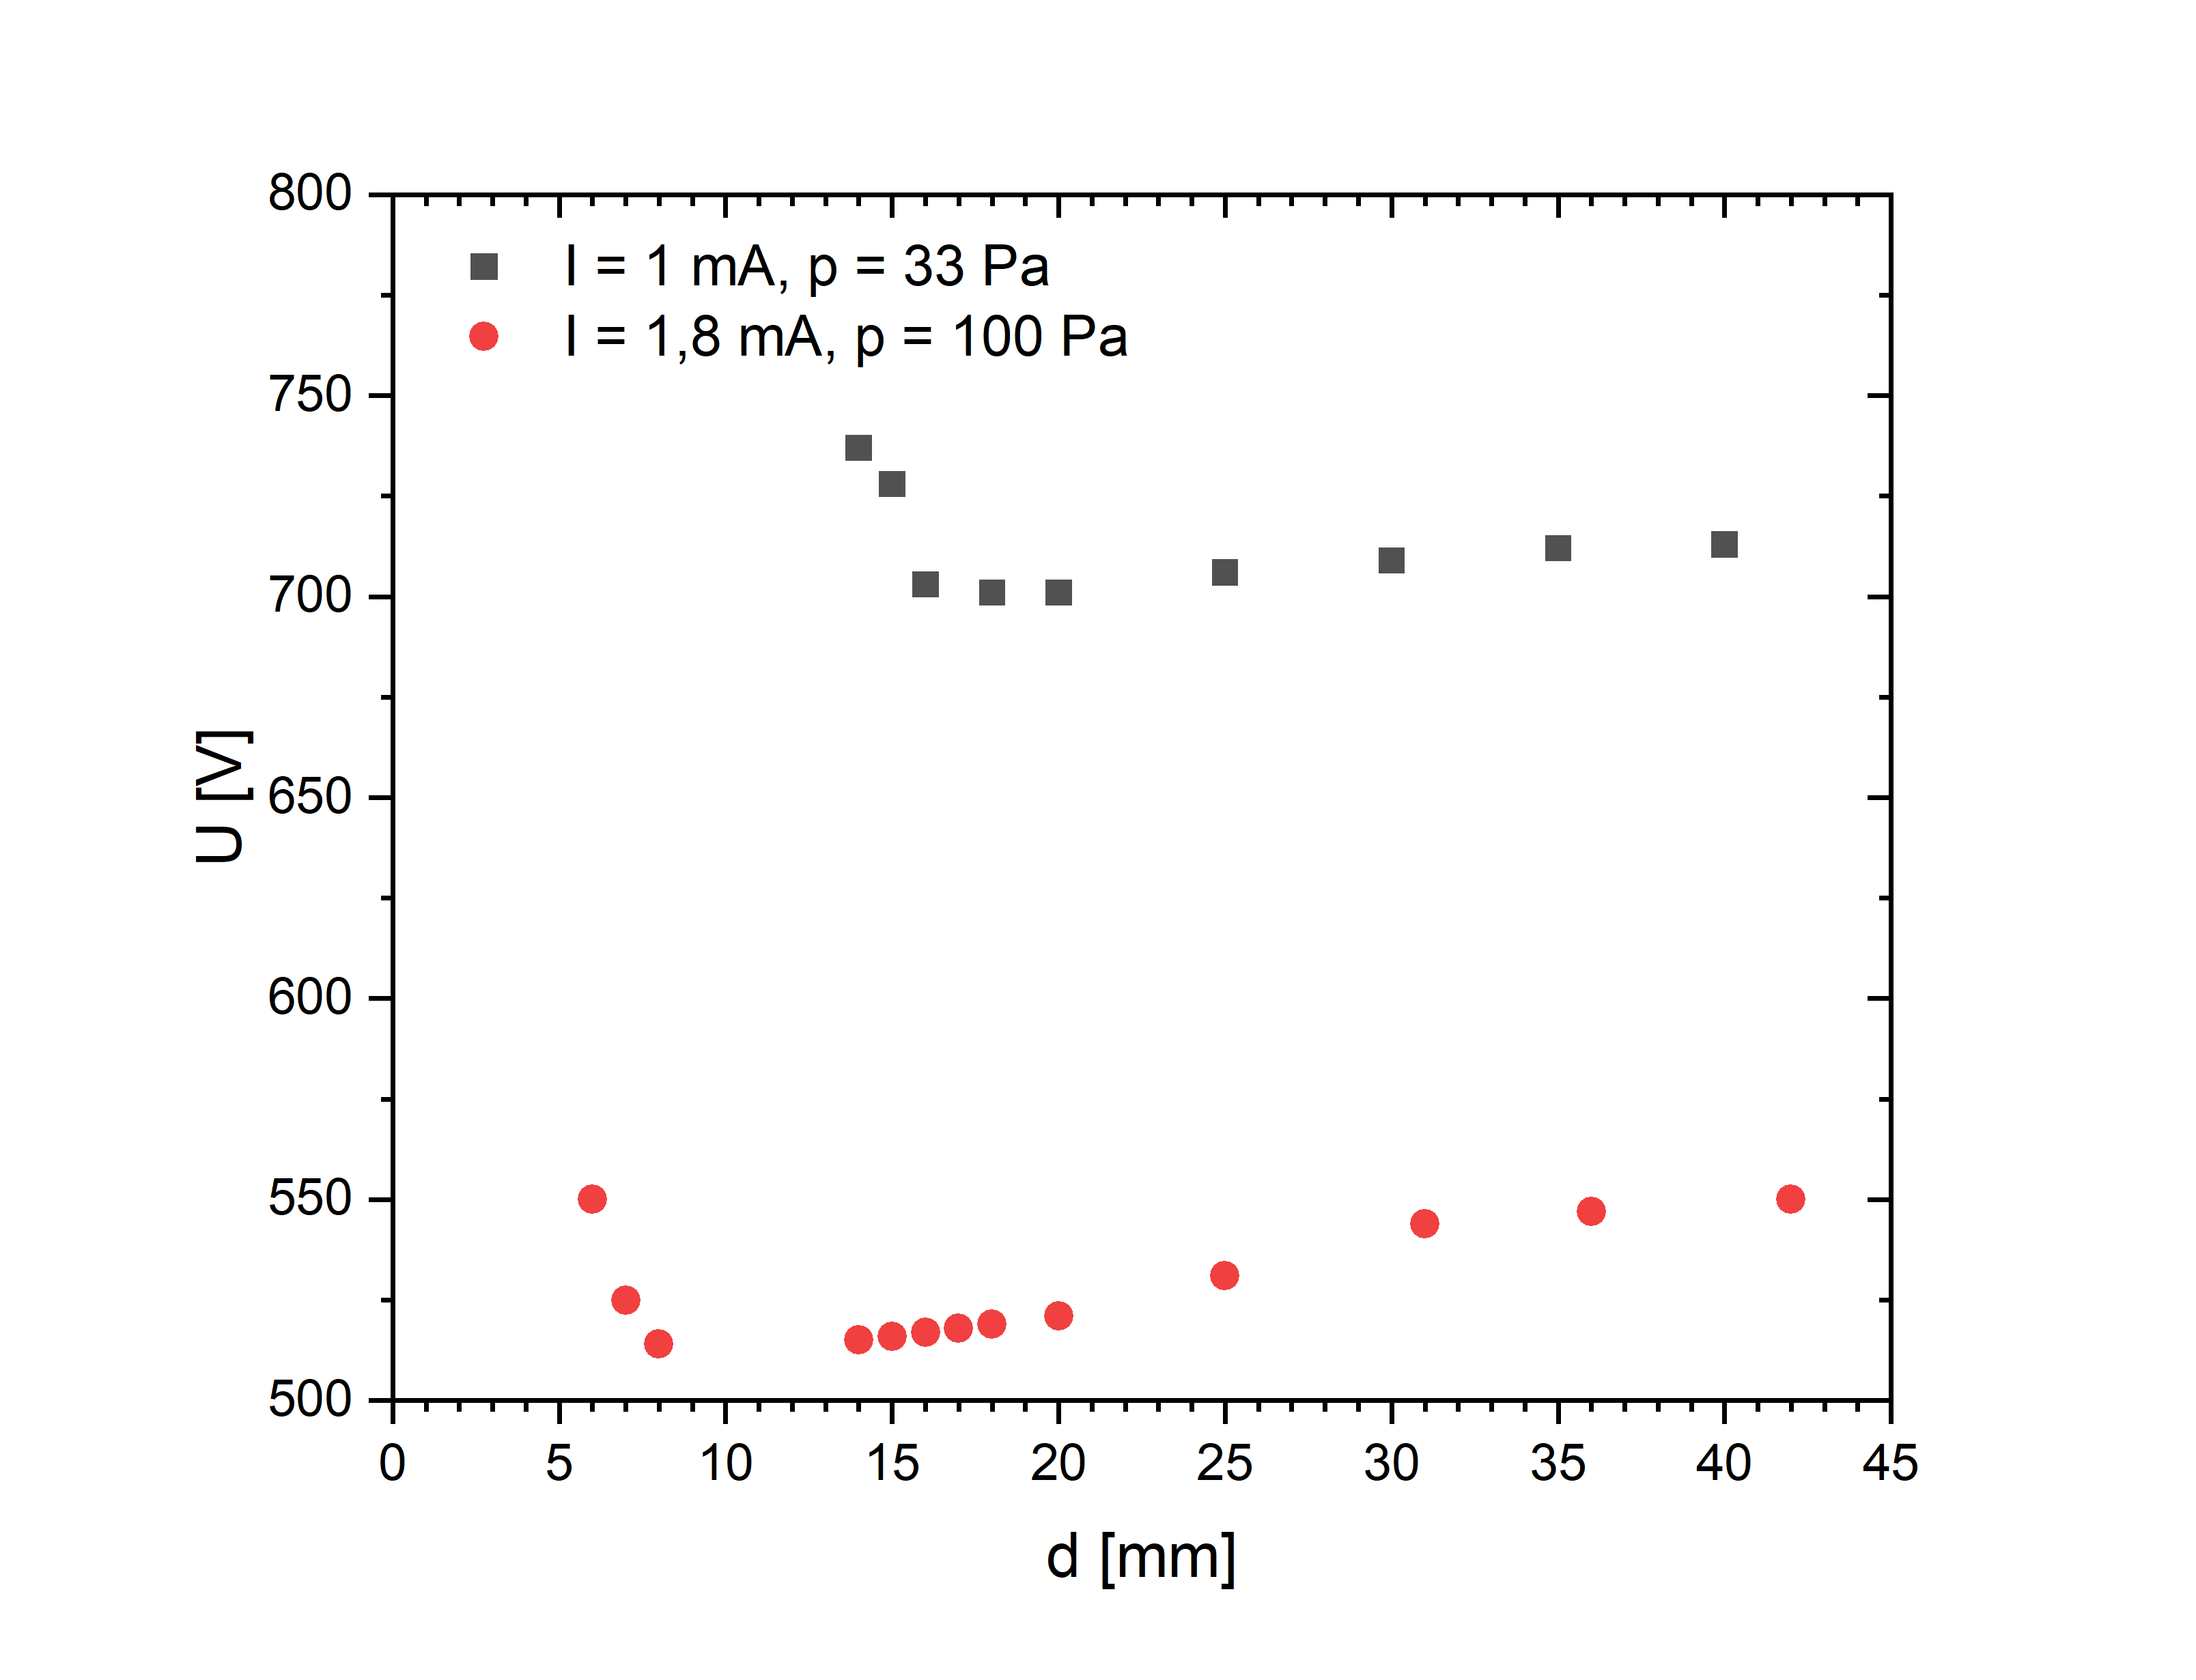
\includegraphics[width=145mm]{KatodovySpad.png}
	\caption{Závislosti napětí na vzdálenosti elektrod, kde minimum napětí odpovídá katodovému spádu.}
	\label{KatodovySpad}
\end{figure}

\newpage
Pro měření voltampérové charakteristiky bylo použito zapojení dle schématu na 
obr.~\ref{schema1}. Naměřená voltampérová charakteristika je v~grafu na 
obr.~\ref{VAodpor}. Vidíme, 
že se nám podařilo naměřit oblast C-E, jak je znázorněno v~obr.~\ref{VA}. 
Oblast C-D se nazývá normální doutnavý výboj. Vyšší proud je kompenzovaný 
zvětšením plochy katodové vrstvy. Až je celý povrch katody pokrytý výbojem, 
zvětšuje 
se velikost katodového spádu, a tím tok iontů na katodu. Tomu odpovídá 
abnormální doutnavý výboj, tedy oblast D-E. Dalším ohřevem katody by výboj 
přešel v~elektrický oblouk.

\begin{figure}[h!]
	\centering
	\includegraphics[width=145mm]{graph1.png}
	\caption{Voltampérová charakteristika}
	\label{VAodpor}
\end{figure}

\clearpage
\section{Závěr}
V~této úloze jsme se seznámili s~Paschenovým zákonem, tedy závislostí zápalného 
napětí na součinu tlaku a vzdálenosti elektrod. Podařilo se nám naměřit typický 
tvar Paschenovy křivky včetně jejího minima. To je důležité pro nejrůznější 
aplikace výbojů, protože se jedná o~bod, ve kterém lze nejsnázeji zapálit výboj.
Dále jsme se zabývali měřením katodového spádu potenciálu. Pro 
$I = 1\,\si{\milli\ampere}$ a $p = 33\,\si{\pascal}$ jsme dostali katodový spád 
$U_\text{k} = 701\,\si{\volt}$. Pro $I = 1,8\,\si{\milli\ampere}$ a $p = 
100\,\si{\pascal}$ je katodový spád nižší,  $U_\text{k} = 514\,\si{\volt}$. 
Zjistili jsme, že oblast katodového spádu je pro hoření výboje kritická. Pokud 
přiblížíme elektrody takových způsobem, že zmizí katodová vrstva, je kvůli 
ztížené ionizaci pro hoření výboje potřeba dodávat vysoké napětí. Nakonec jsme 
naměřili voltampérovou charakteristiku doutnavého výboje, kterou jsme 
identifikovali jako oblasti odpovídající normálnímu i abnormálnímu doutnavému 
výboji.

\begin{thebibliography}{10}
	\bibitem{wiki}
	Wikipedia contributors. Paschen's law [Internet]. Wikipedia, The Free 
	Encyclopedia; 2022 Mar 31, 05:42 UTC [cited 2022 Apr 27]. Available from: 
	\url{https://en.wikipedia.org/w/index.php?title=Paschen%27s_law&oldid=1080258746.}

\end{thebibliography}

\end{document}
